\chapter{Testing - "Testing and evaluation"}


\section{Introduction}

With every new line of code, comes the potential of a new bug. Testing the code makes for a better built and reliable application. The type of testing undertaken for this application was functional testing. 

\section{Testing the Homepage}

\subsection{Functional Testing}

Testing initiated with the homepage. Within the navigation bar at the top of the page, all links were checked in order to ensure that the user was brought to the correct link. In addition to this ensuring that the pages were loaded without any errors. The only errors which should be generated are those that are intentional. Intentional errors are included in figure \ref{fig:Intentional Error Register} and \ref{fig:Intentional Error Login}. This shows that the code was doing what it was meant to do.

\begin{figure}[htbp]
   \centering
   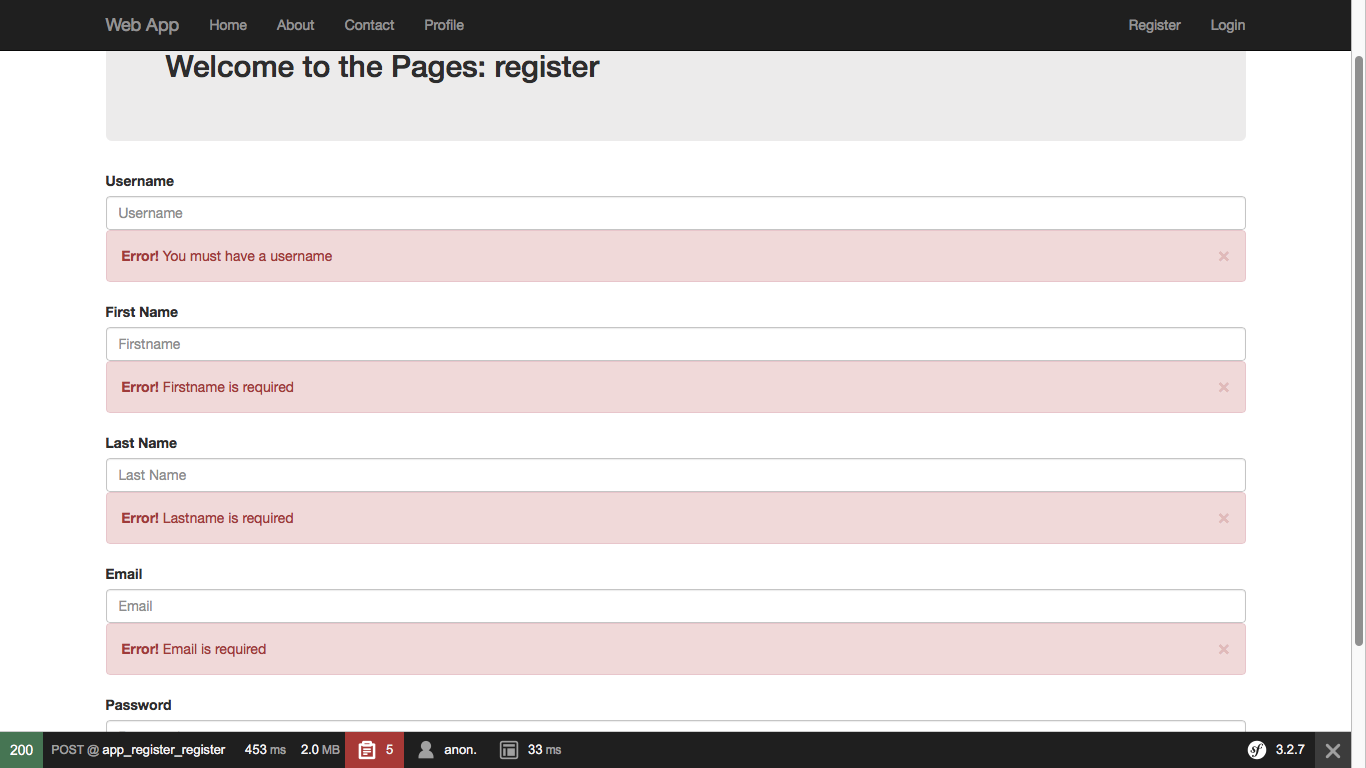
\includegraphics[width=400pt]{figures/intentional_error_register.png} % requires the graphicx package
   \caption{Intentional Error Register}
   \label{fig:Intentional Error Register}
\end{figure}

\begin{figure}[htbp]
   \centering
   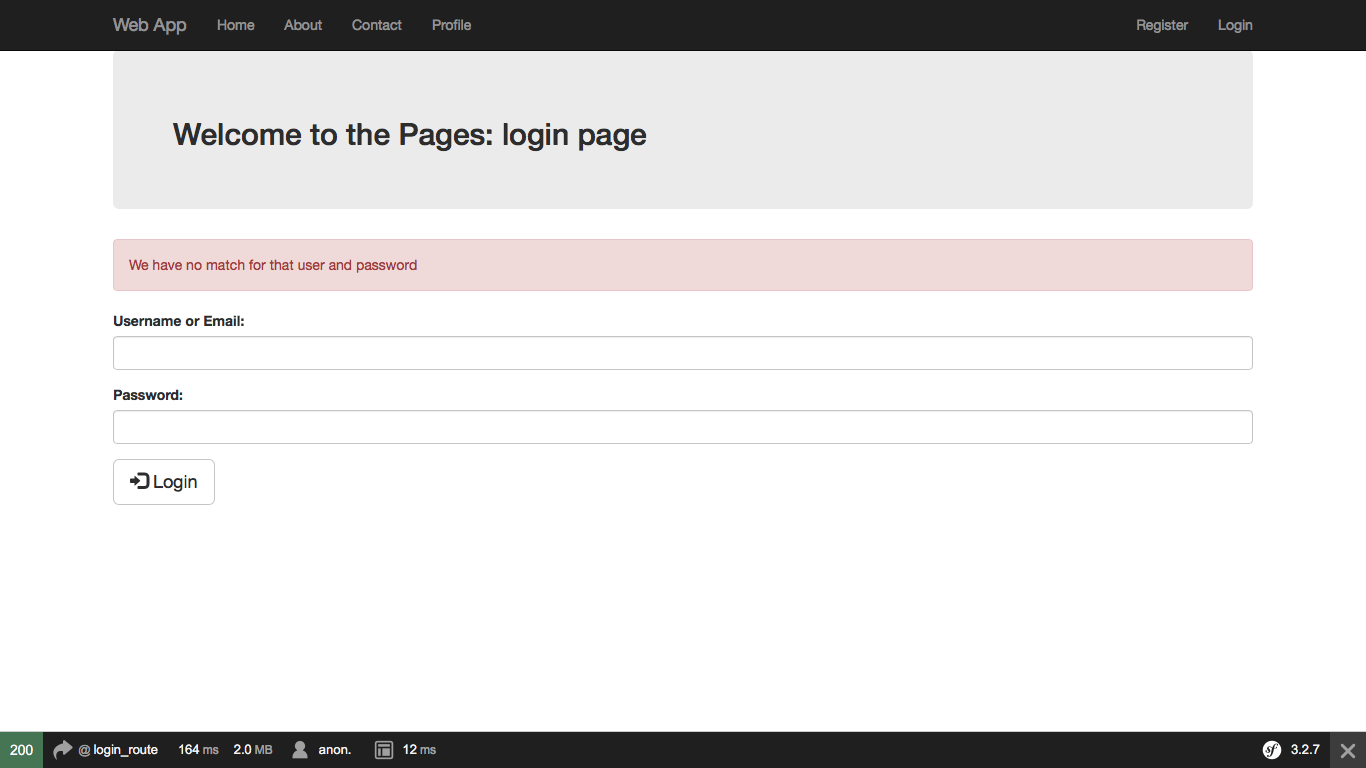
\includegraphics[width=400pt]{figures/intentional_error_login.png} % requires the graphicx package
   \caption{Intentional Error Login}
   \label{fig:Intentional Error Login}
\end{figure}

Errors are shown in the Symfony debug toolbar figure \ref{fig:Debug Error Register} and if one looks at the profiler it was clear that credentials were not provided by the user. Figure \ref{fig:Profiler Error Register}.

\begin{figure}[htbp]
   \centering
   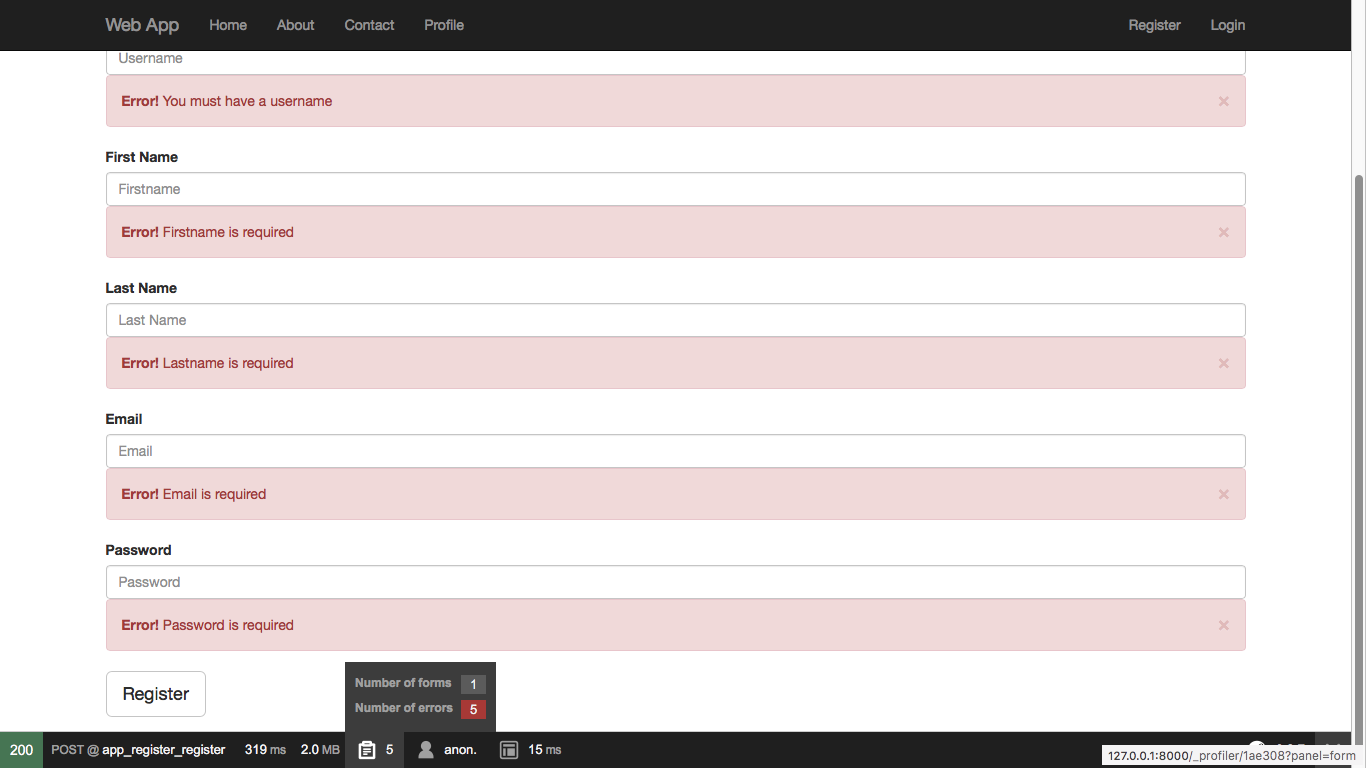
\includegraphics[width=400pt]{figures/profiler_intentional_error_register.png} % requires the graphicx package
   \caption{Debug Error Register}
   \label{fig:Debug Error Register}
\end{figure}

\begin{figure}[htbp]
   \centering
   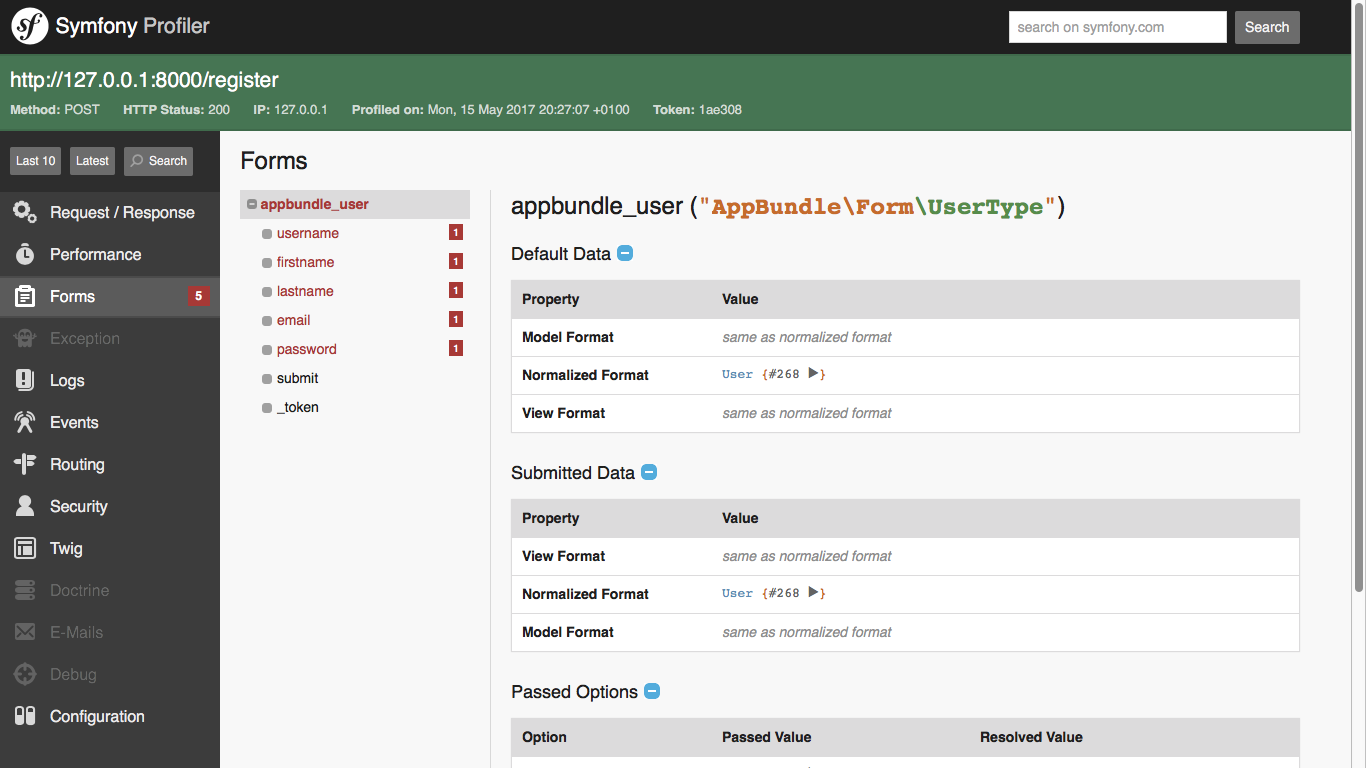
\includegraphics[width=400pt]{figures/profiler_error_register.png} % requires the graphicx package
   \caption{Profiler Error Register}
   \label{fig:Profiler Error Register}
\end{figure}

\section{Testing Registration}

\subsection{Successful Registration}

Although the user enters their details into the form. Nothing might come of it. Which means the form was not handled correctly. This was why informing the user on the client side was important. It gives them some indication that the action which they performed had the potential to be a success figure \ref{fig:Successful Registration}.

\begin{figure}[htbp]
   \centering
   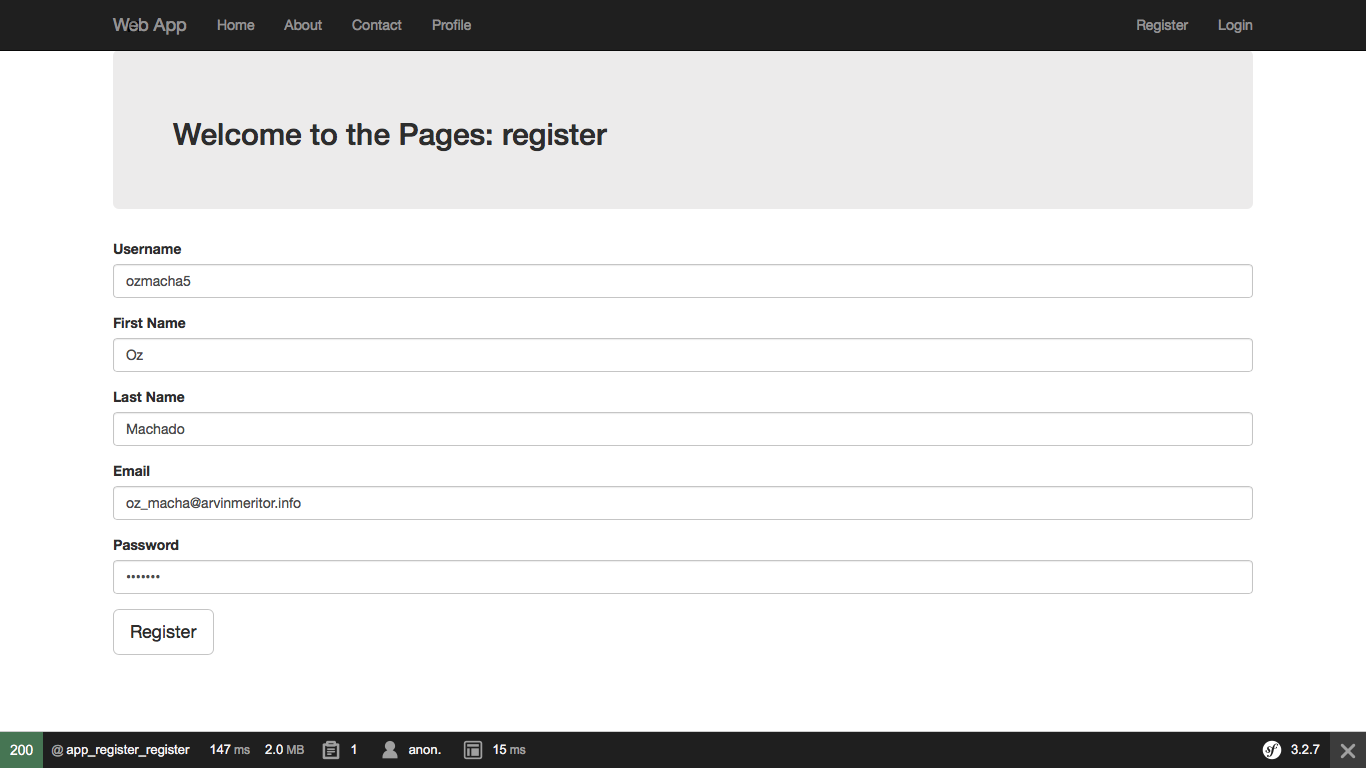
\includegraphics[width=400pt]{figures/register_check.png} % requires the graphicx package
   \caption{Register Test}
   \label{fig:Register Test}
\end{figure}

\begin{figure}[t]
   \centering
   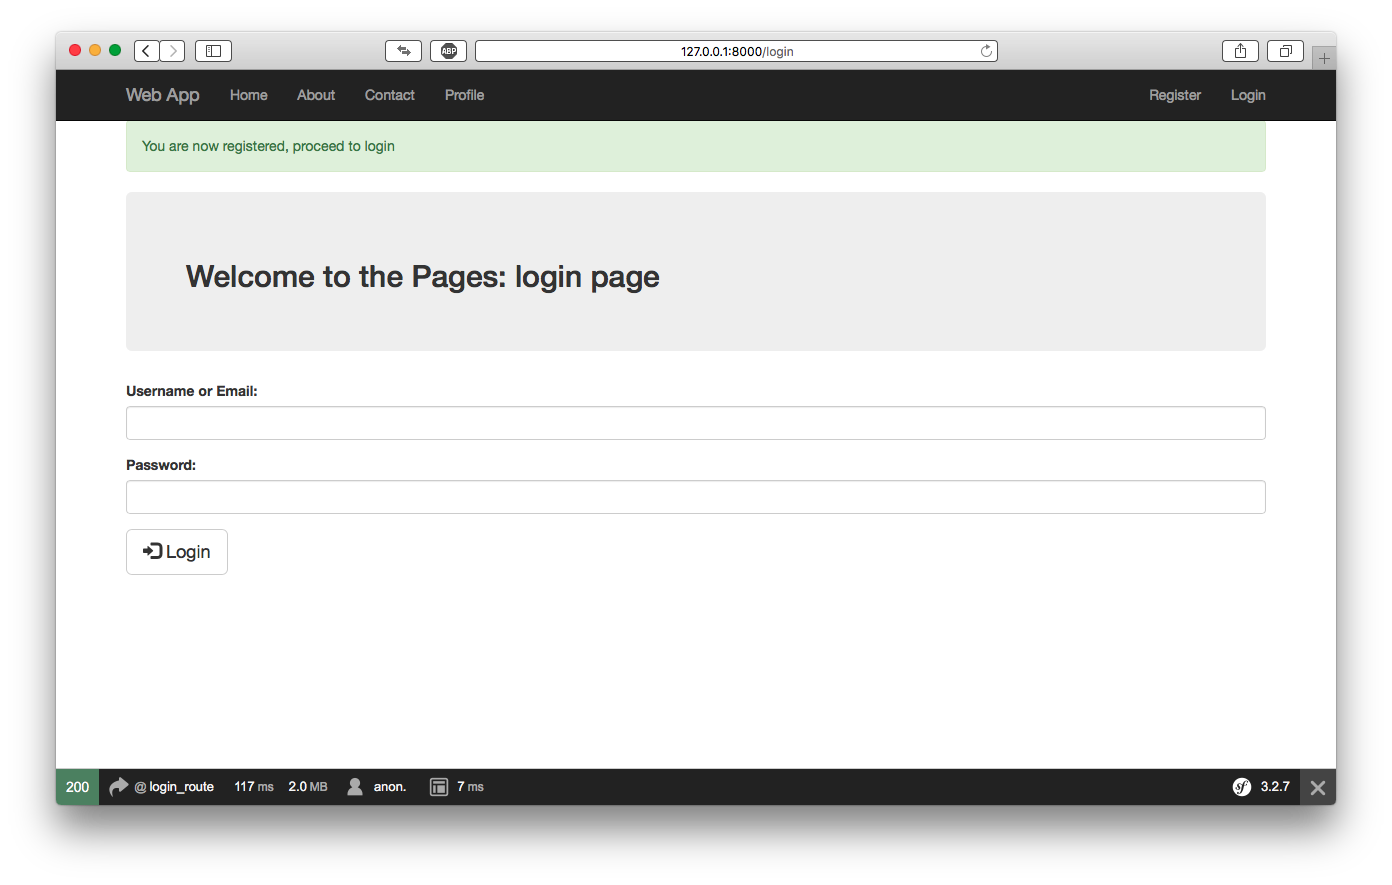
\includegraphics[width=400pt]{figures/register_successful.png} % requires the graphicx package
   \caption{Successful Registration}
   \label{fig:Successful Registration}
\end{figure}

On the server side it was possible to view what the user entered into the form \ref{fig:Database Check} and give the role of ROLE USER in the role field.

\begin{figure}[htbp]
   \centering
   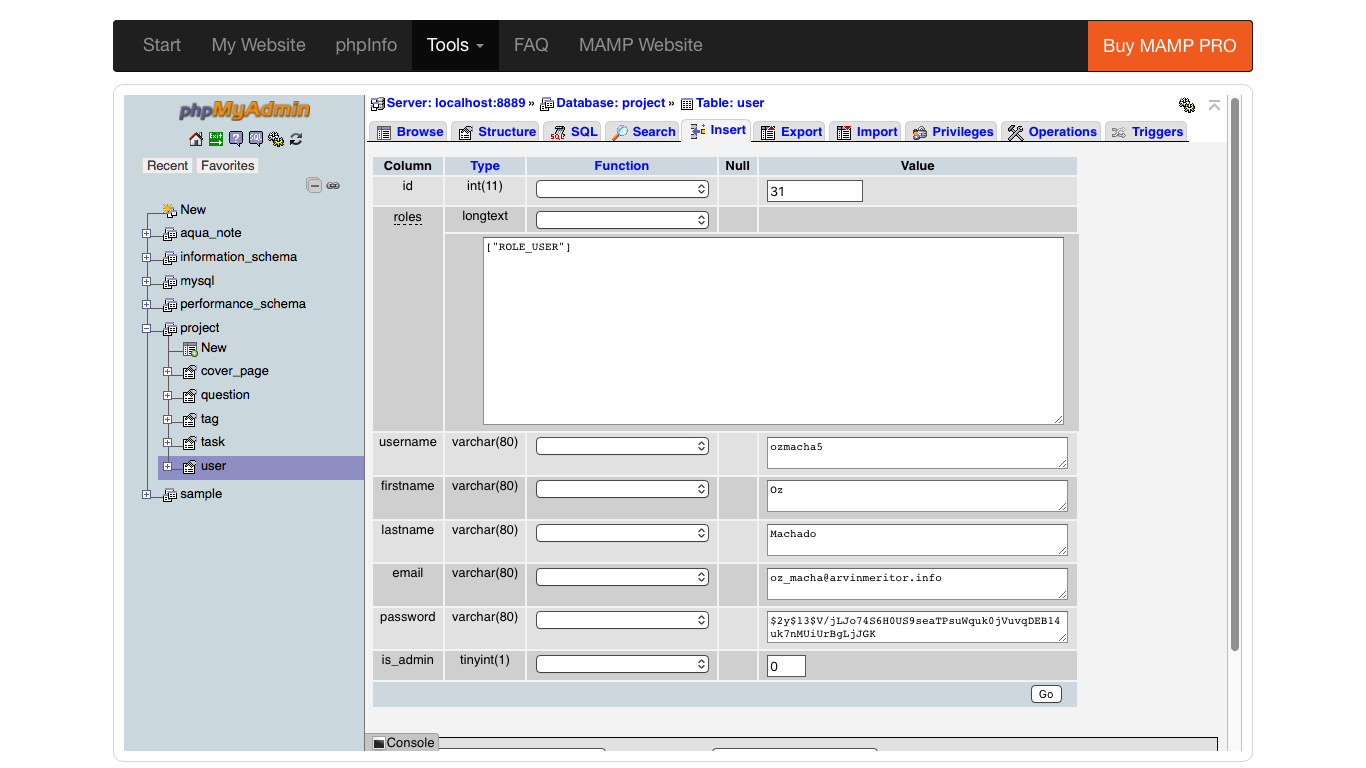
\includegraphics[width=400pt]{figures/db_check.png} % requires the graphicx package
   \caption{Database Check}
   \label{fig:Database Check}
\end{figure}

%\clearpage

\section{Testing Login}

\subsection{Successful Login}

In figure \ref{fig:Mr Oz Machado Login} this guarantees the user that it was a success as they are successfully logged in and authenticated.

\begin{figure}[htbp]
   \centering
   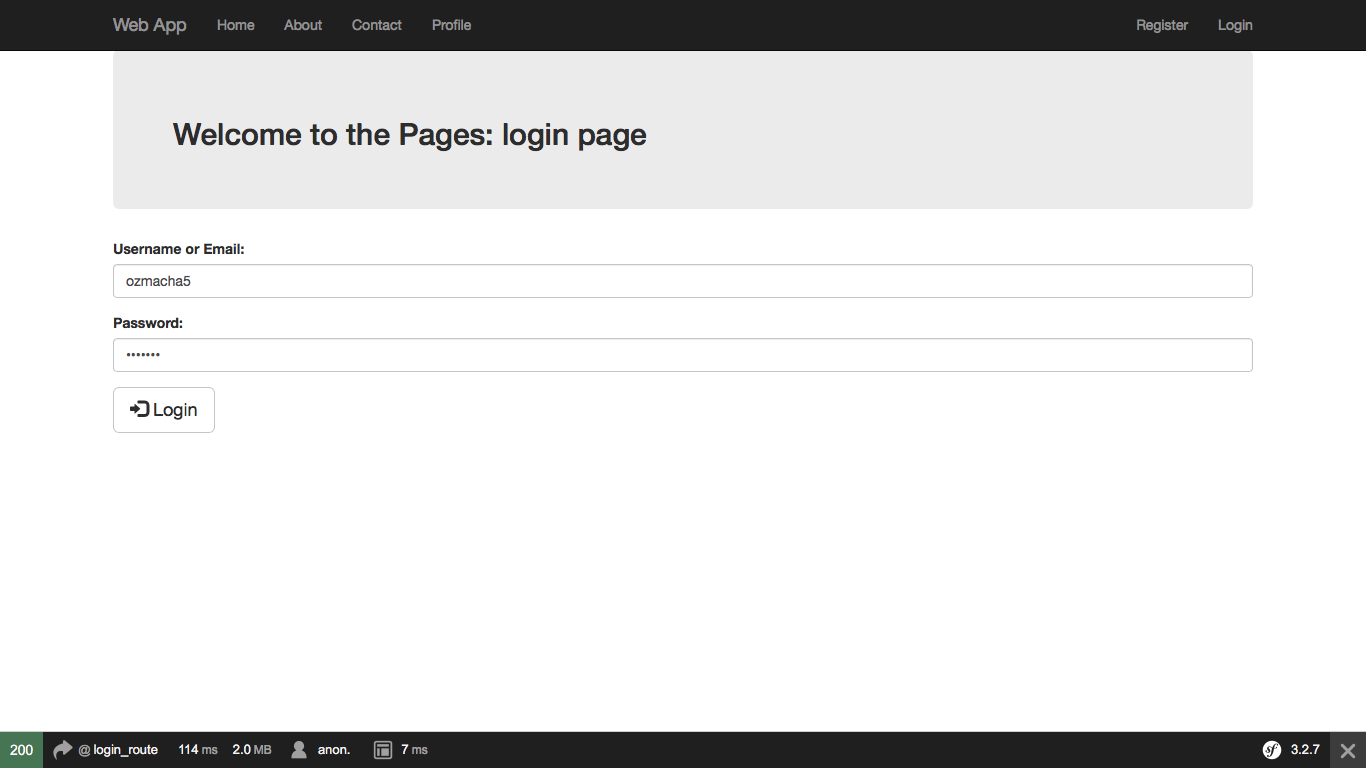
\includegraphics[width=400pt]{figures/ozmacha5_login.png} % requires the graphicx package
   \caption{Mr Oz Machado Login}
   \label{fig:Mr Oz Machado Login}
\end{figure}

\begin{figure}[htbp]
   \centering
   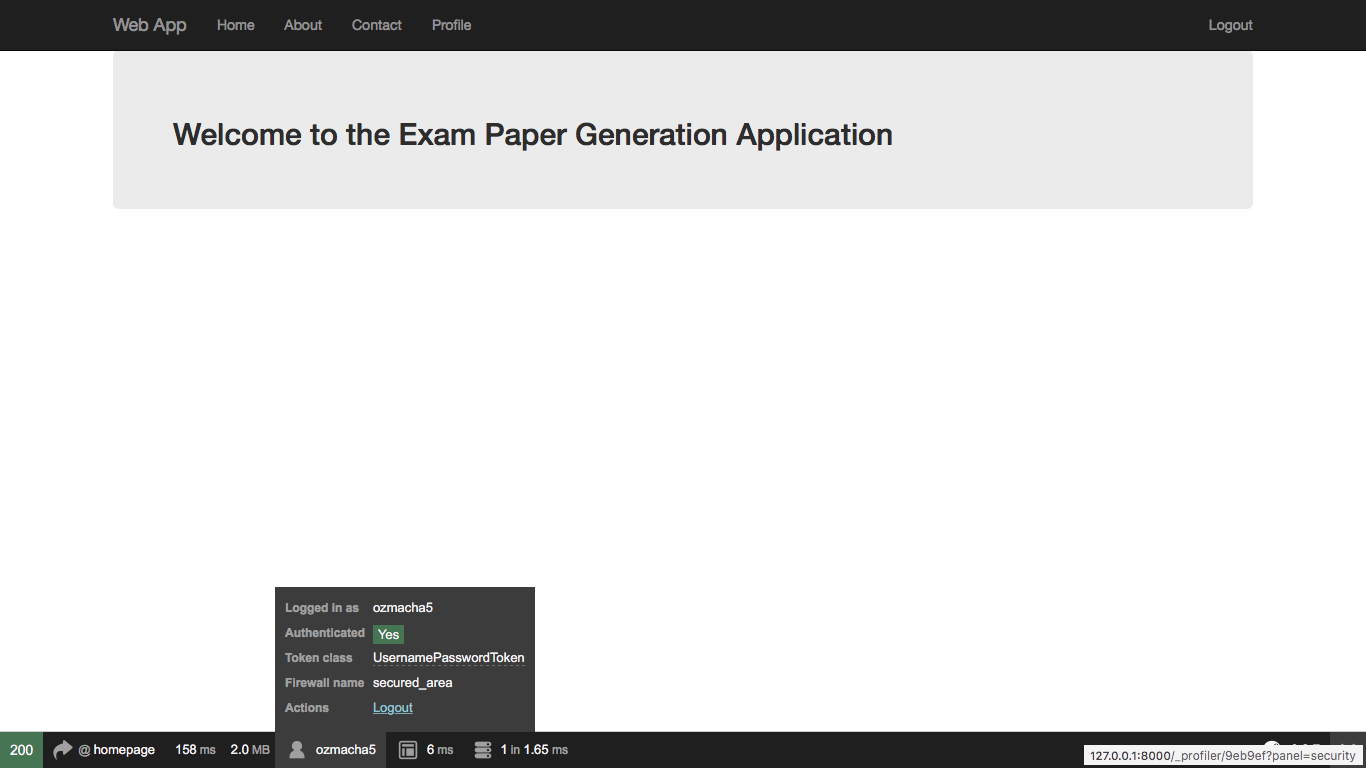
\includegraphics[width=400pt]{figures/ozmacha5_success.png} % requires the graphicx package
   \caption{Oz Machado Authenticated}
   \label{fig:Oz Machado Authenticated}
\end{figure}

As an administrator it was possible to view the recently added user to give confirmation that the application was working as it should.

%\clearpage

\begin{figure}[htbp]
   \centering
   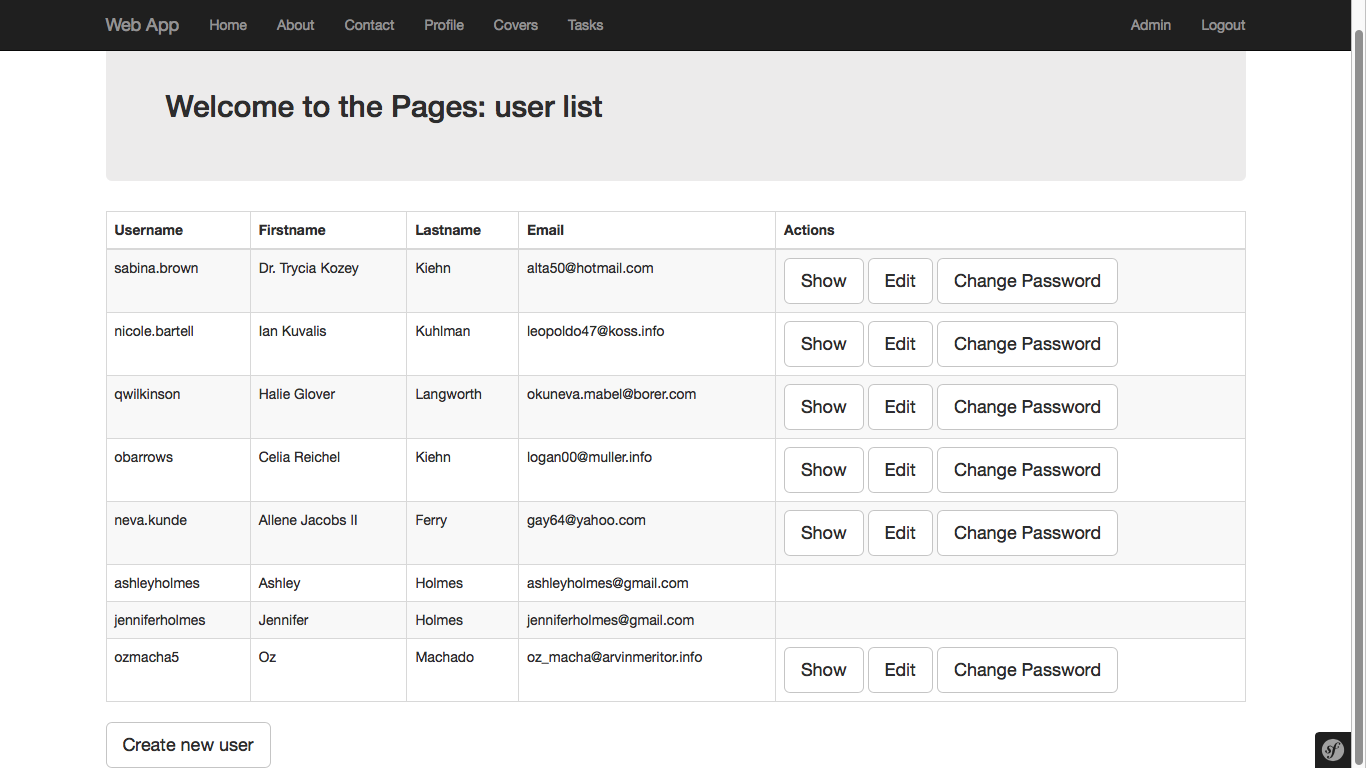
\includegraphics[width=400pt]{figures/ozmacha5_index.png} % requires the graphicx package
   \caption{Oz Machado Index Page}
   \label{fig:Oz Machado Index Page}
\end{figure}

\begin{figure}[htbp]
   \centering
   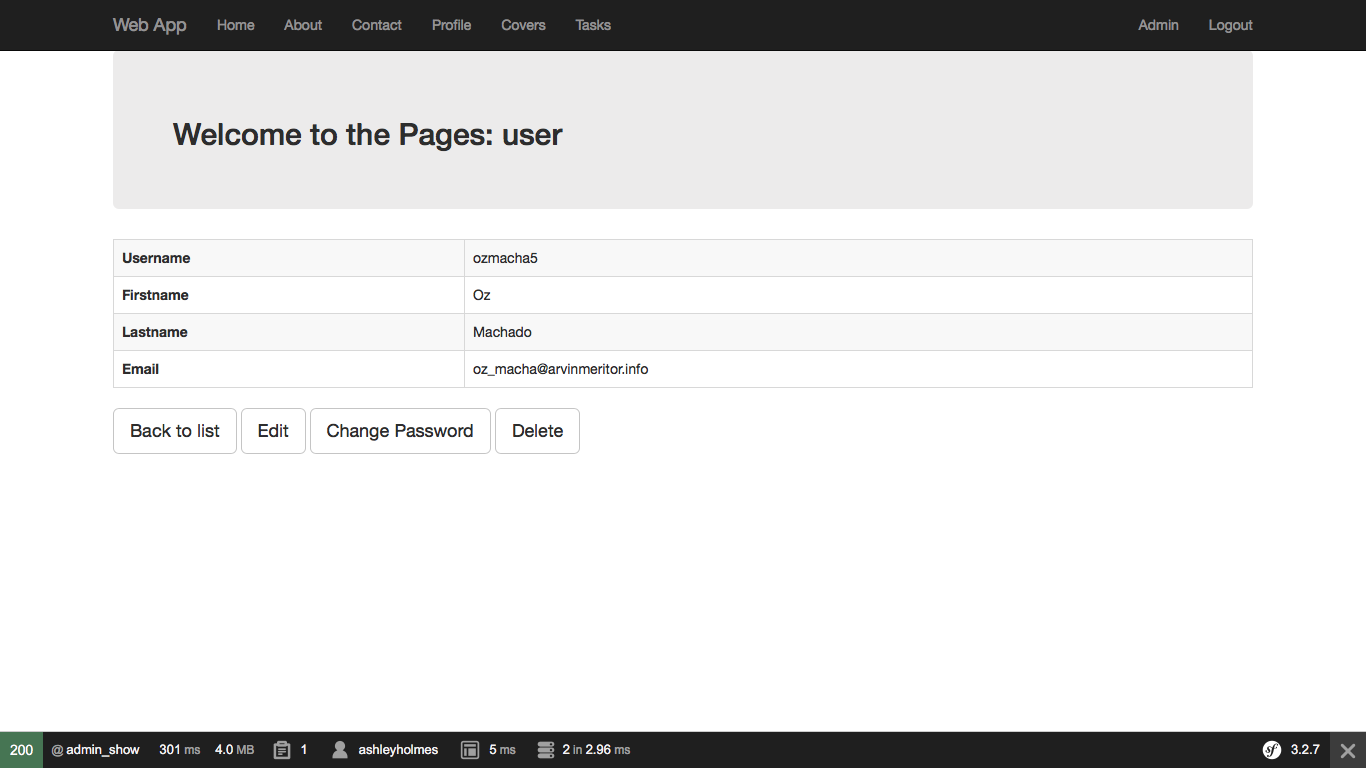
\includegraphics[width=400pt]{figures/ozmacha5_show.png} % requires the graphicx package
   \caption{Oz Machado Show Page}
   \label{fig:Oz Machado Show Page}
\end{figure}

\section{Testing Editing}

\subsection{Successful Editing Function}

In figure \ref{fig:Oz Name Changed} it was clear that the edit method was functioning correctly. As the first name of the user was successfully changed to the Wizard of Oz. 

\begin{figure}[htbp]
   \centering
   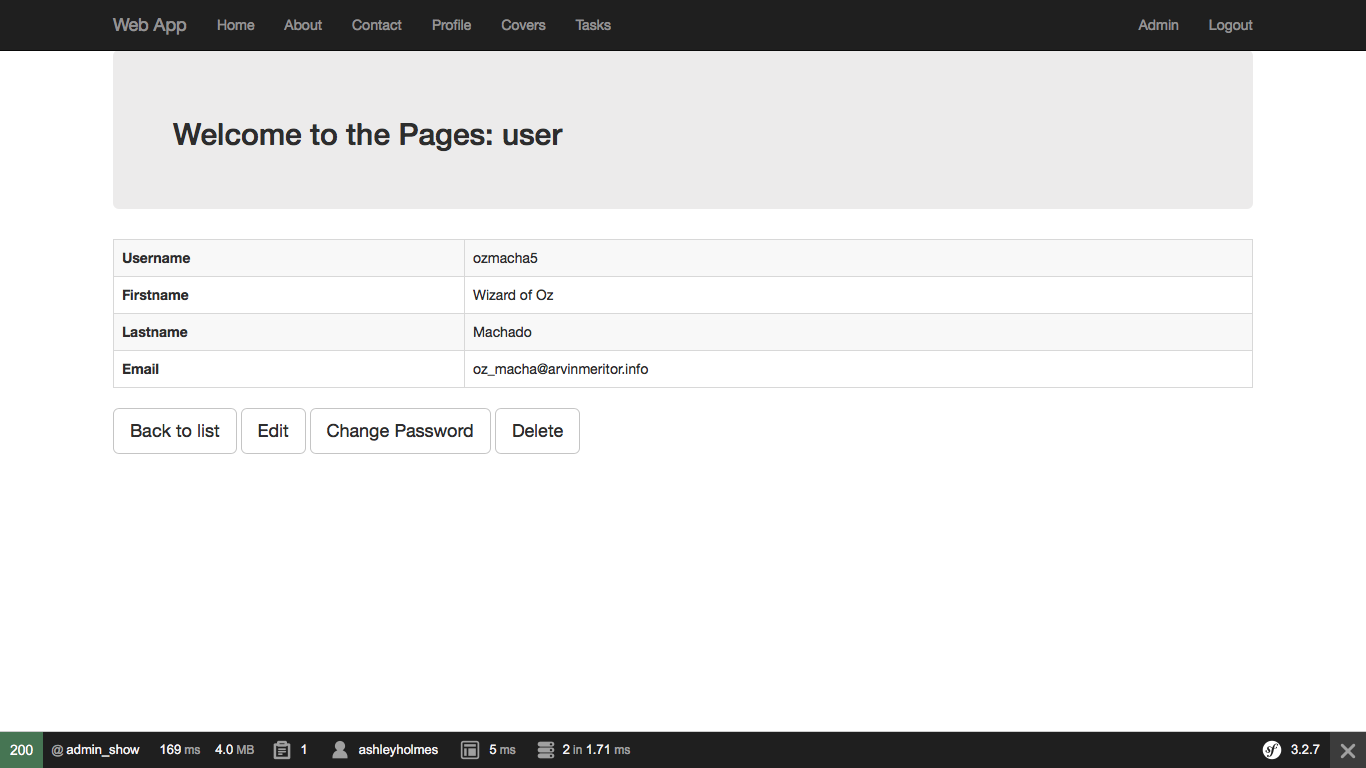
\includegraphics[width=400pt]{figures/wizard_oz.png} % requires the graphicx package
   \caption{Oz Name Changed}
   \label{fig:Oz Name Changed}
\end{figure}

%\clearpage

\section{Testing Password}

\subsection{Successful Password Editing}

Here the users password was changed. This cannot be seen in the password view yet this change can be seen in the database in the password field. The encryption pattern on the password is different to the figure \ref{fig:Database Check}.

\begin{figure}[htbp]
   \centering
   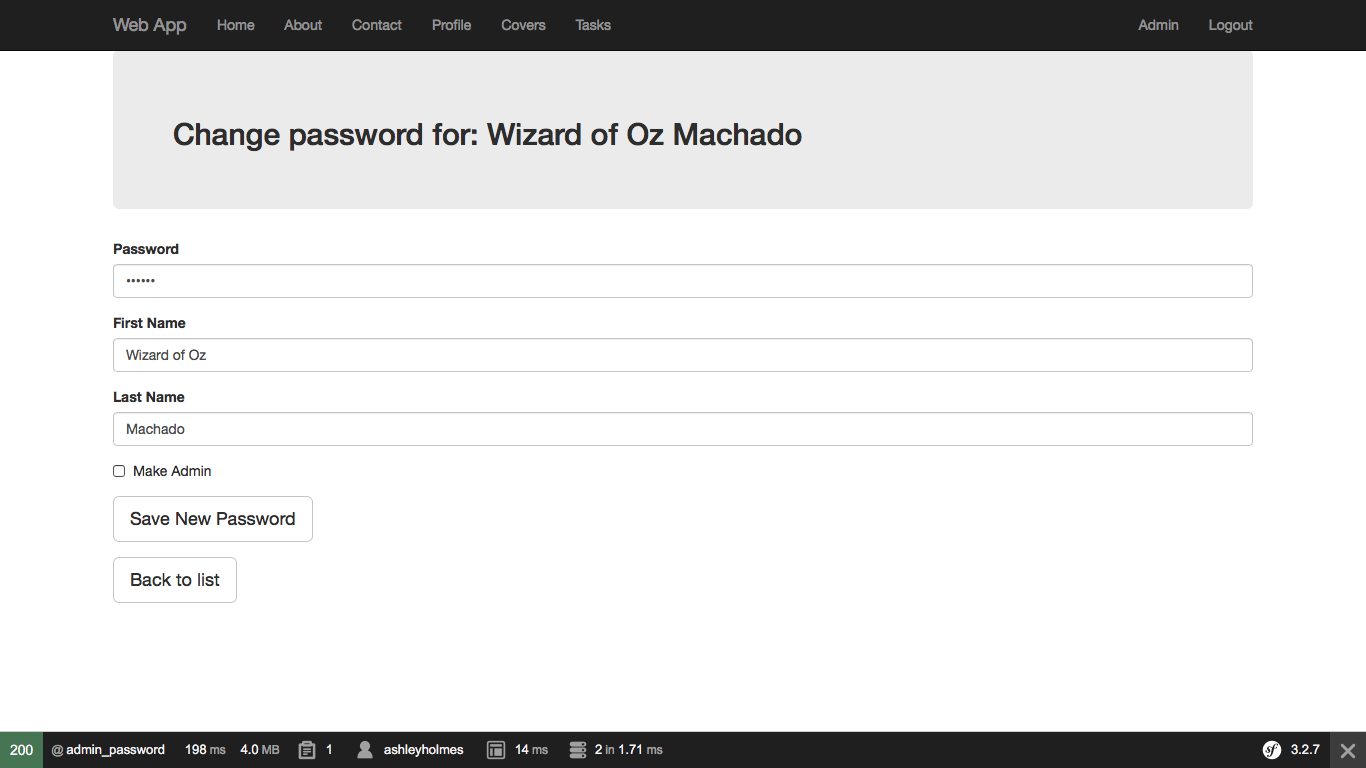
\includegraphics[width=400pt]{figures/oz_change_password.png} % requires the graphicx package
   \caption{Oz Password Changed}
   \label{fig:Oz Password Changed}
\end{figure}

\begin{figure}[htbp]
   \centering
   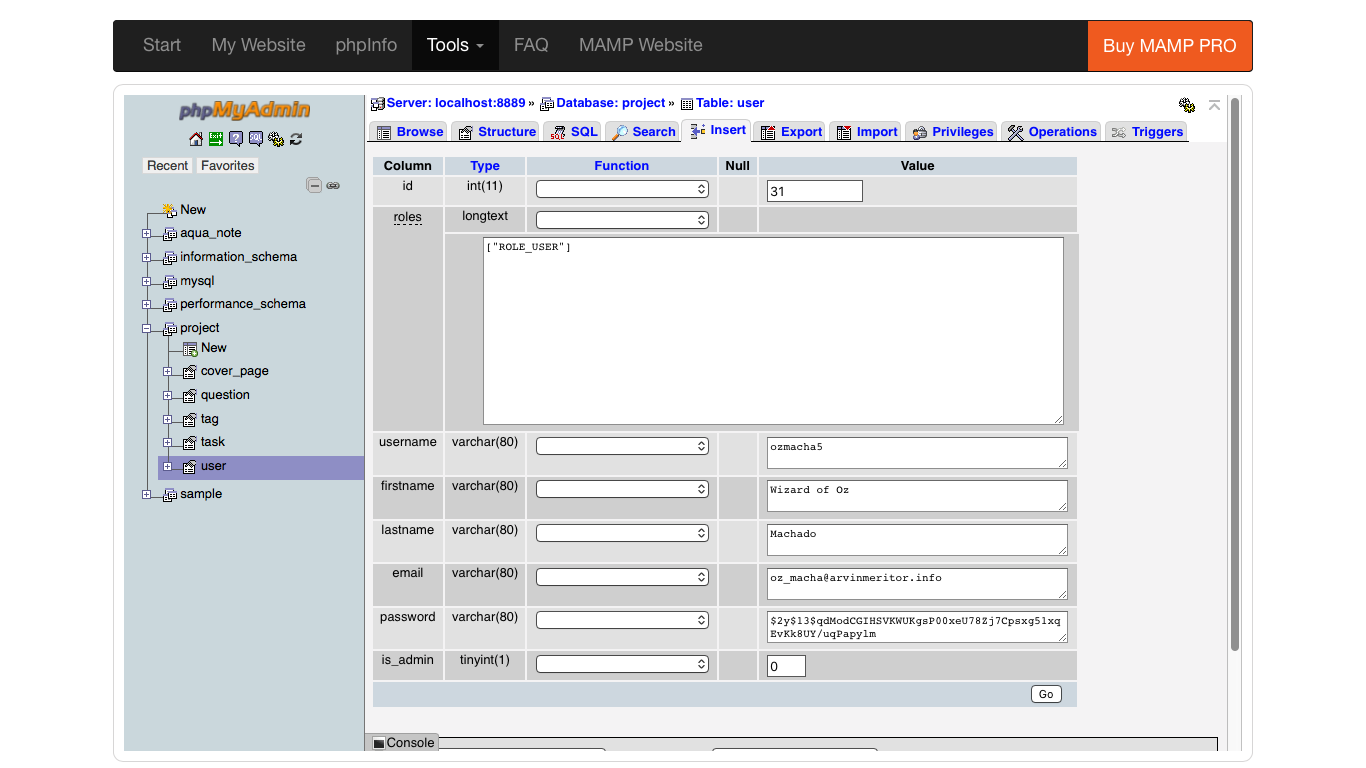
\includegraphics[width=400pt]{figures/oz_change_password_db.png} % requires the graphicx package
   \caption{Oz Password Changed DB}
   \label{fig:Oz Password Changed DB}
\end{figure}

%\clearpage

\section{Testing ROLES}

\subsection{ROLE Changes}

Mr Oz Machado had his ROLE changed from a user role to an admin role which it seen in the roles field in figure \ref{fig:Oz ROLES Changed}. This operation was a success which was indicated by the change made in the database. Which gave him addition rights across the application.

\begin{figure}[htbp]
   \centering
   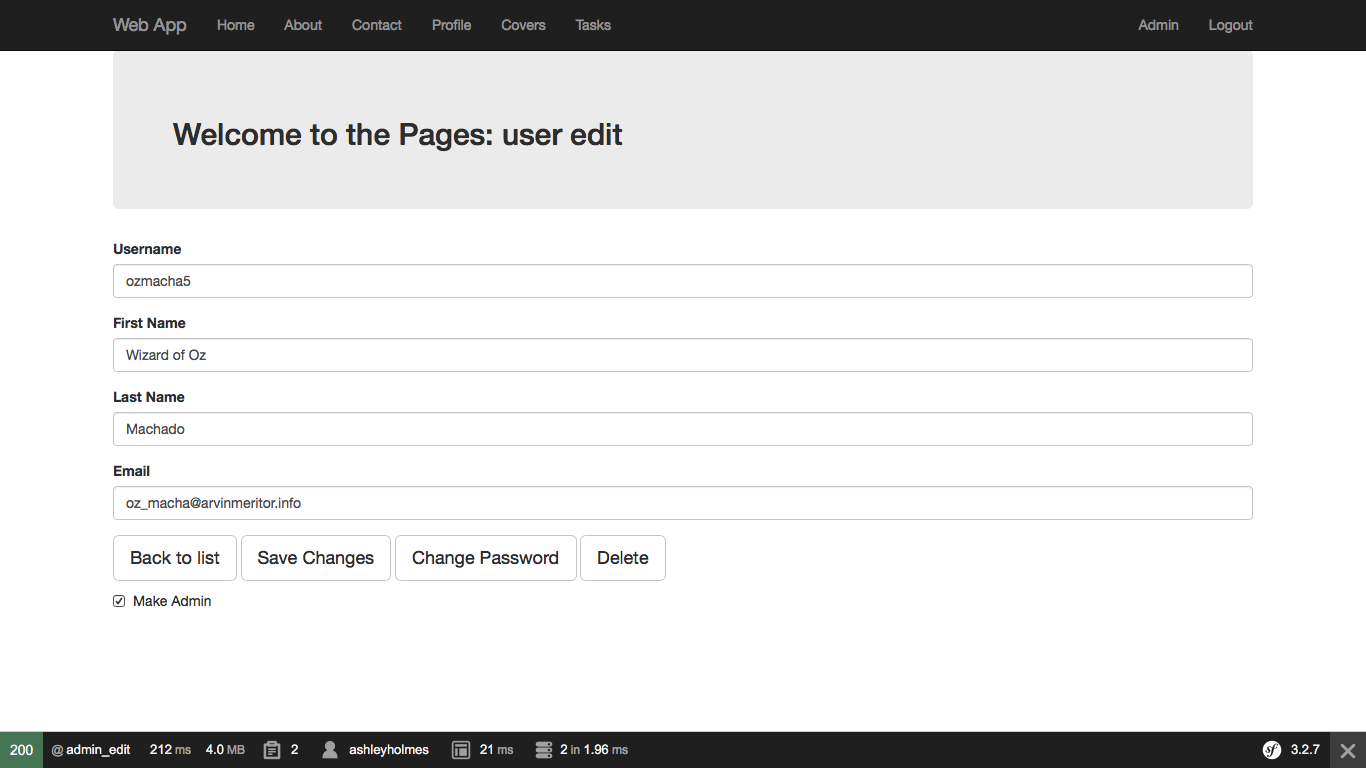
\includegraphics[width=400pt]{figures/oz_making_admin.png} % requires the graphicx package
   \caption{Oz ROLES Changed}
   \label{fig:Oz ROLES Changed}
\end{figure}

\begin{figure}[htbp]
   \centering
   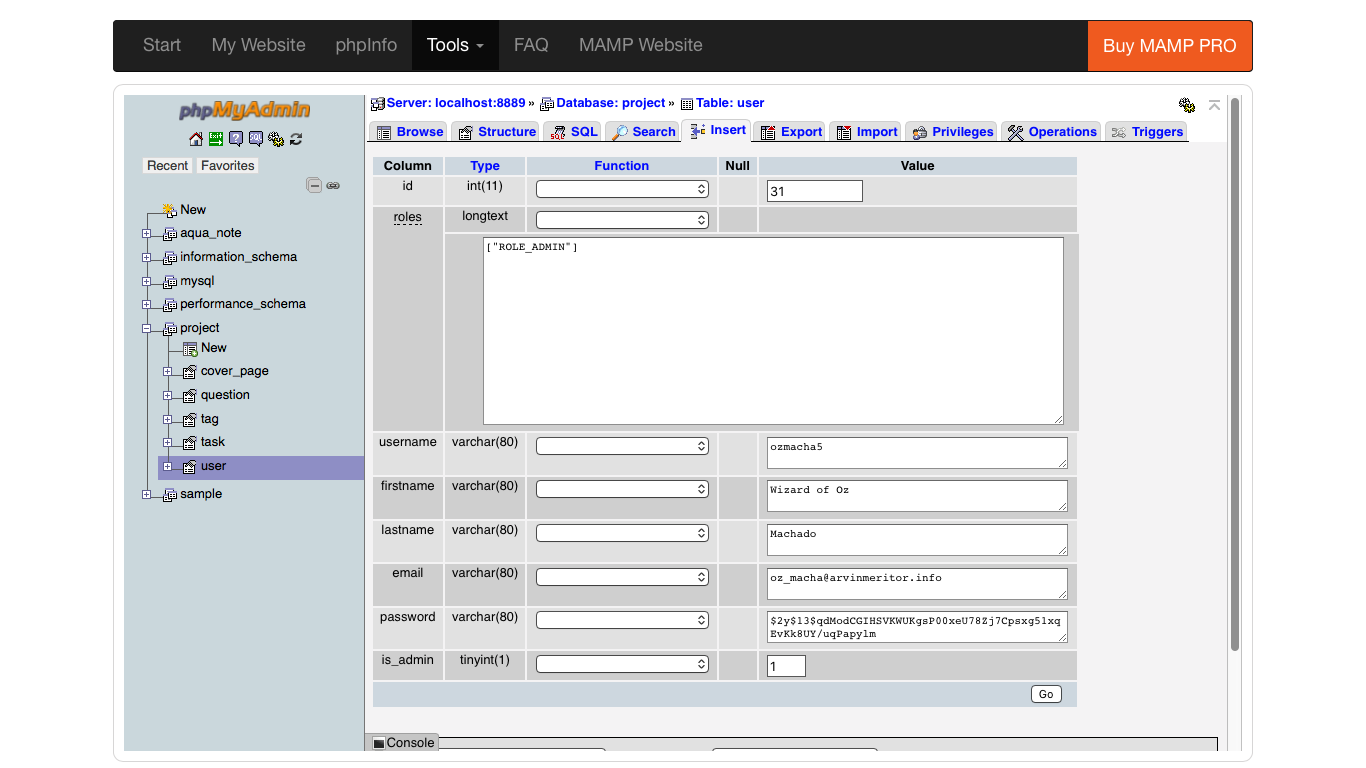
\includegraphics[width=400pt]{figures/oz_making_admin_db.png} % requires the graphicx package
   \caption{Oz ROLES Changed in DB}
   \label{fig:Oz ROLES Changed in DB}
\end{figure}

%\clearpage

\section{Testing Exam Cover Page}

\subsection{Successful Form Validation}

The form validation of the cover page was successful. The user was not able proceed after submitting the form without populating all fields. The errors are specified, explaining to the user what to follow with next. Once successfully completing the form the user was directed back to the admin and the information transferred to the database successfully. The indication of this are in figures \ref{fig:Cover Form Validation}, \ref{fig:Cover Generation Step 1}, \ref{fig:Cover Generation Step 2}, \ref{fig:Cover Generation Step 3}, \ref{fig:Cover Generation Step 4}, \ref{fig:Cover Page Successful} and \ref{fig:Cover Page Successful DB}.

\begin{figure}[htbp]
   \centering
   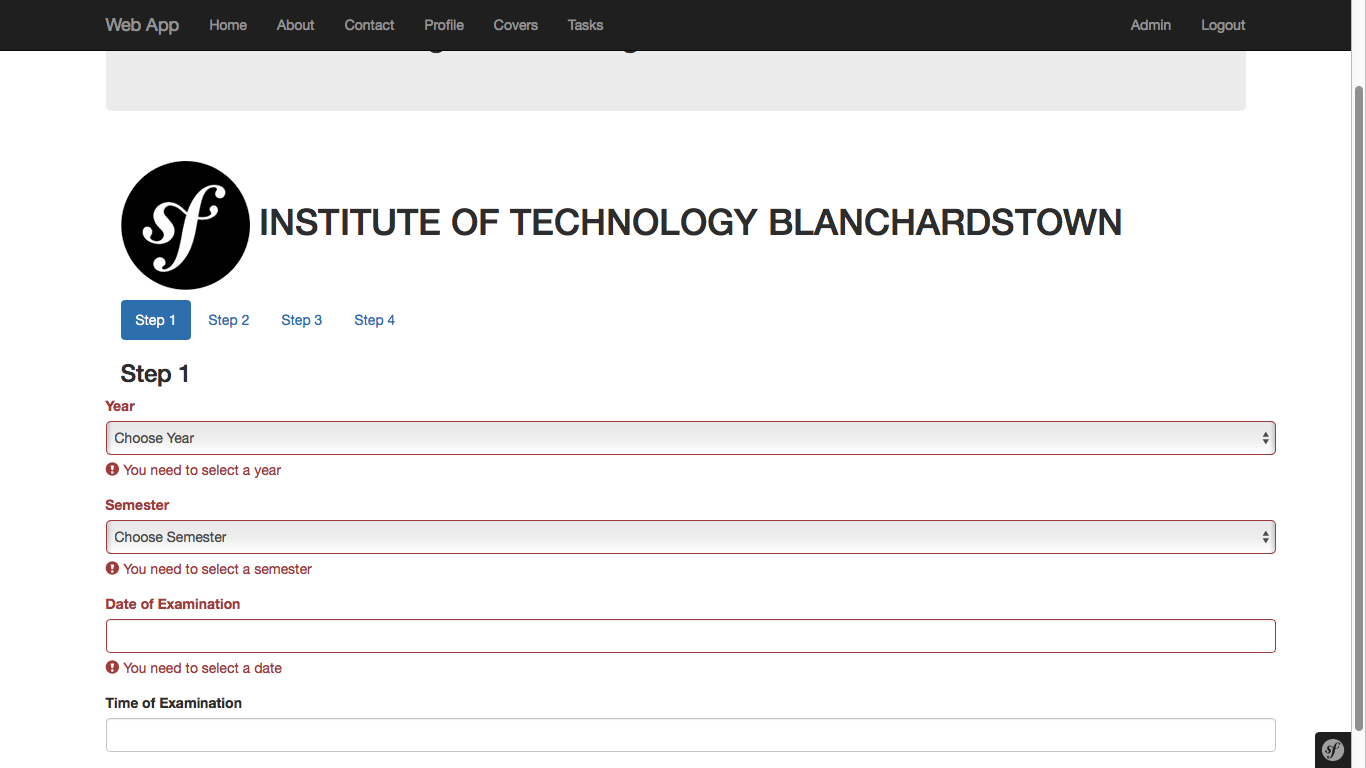
\includegraphics[width=400pt]{figures/covers_test.png} % requires the graphicx package
   \caption{Cover Form Validation}
   \label{fig:Cover Form Validation}
\end{figure}

\begin{figure}[htbp]
   \centering
   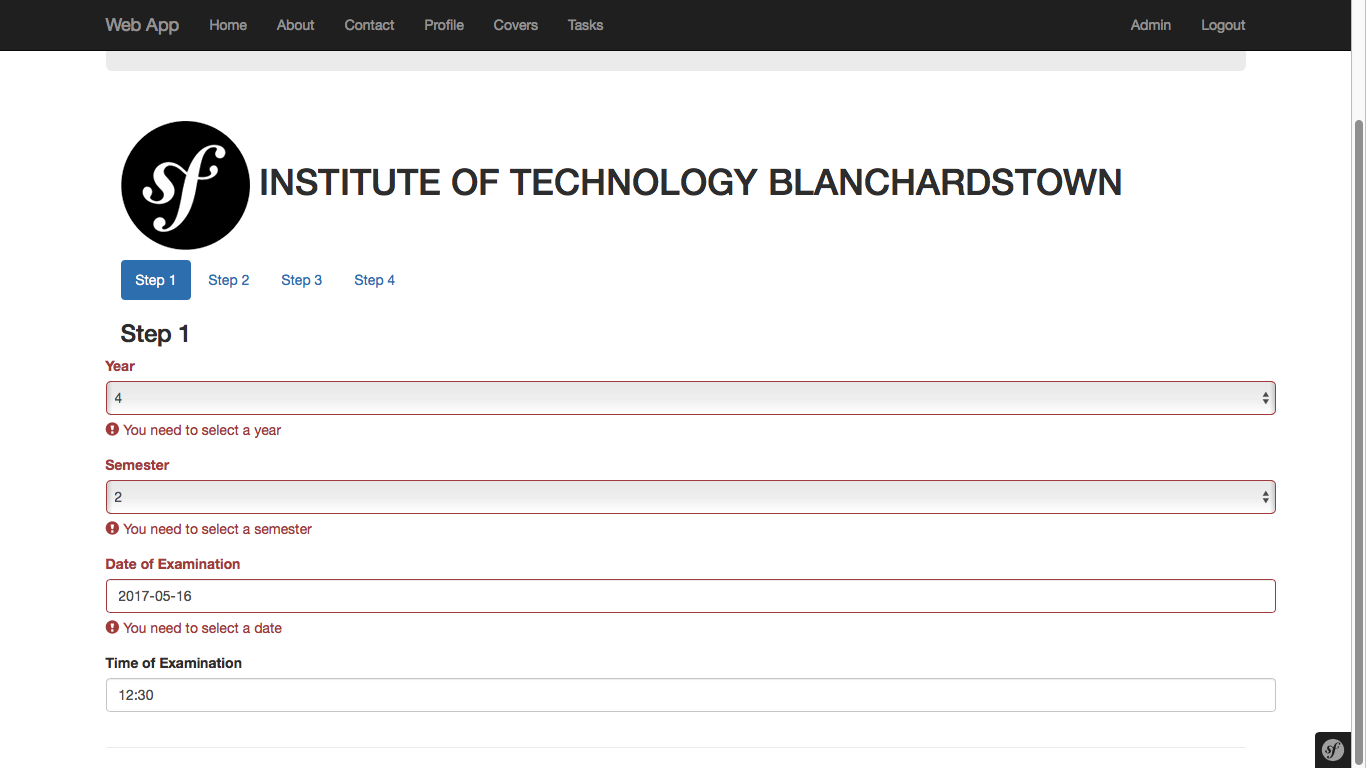
\includegraphics[width=400pt]{figures/step_1.png} % requires the graphicx package
   \caption{Cover Generation Step 1}
   \label{fig:Cover Generation Step 1}
\end{figure}

\begin{figure}[htbp]
   \centering
   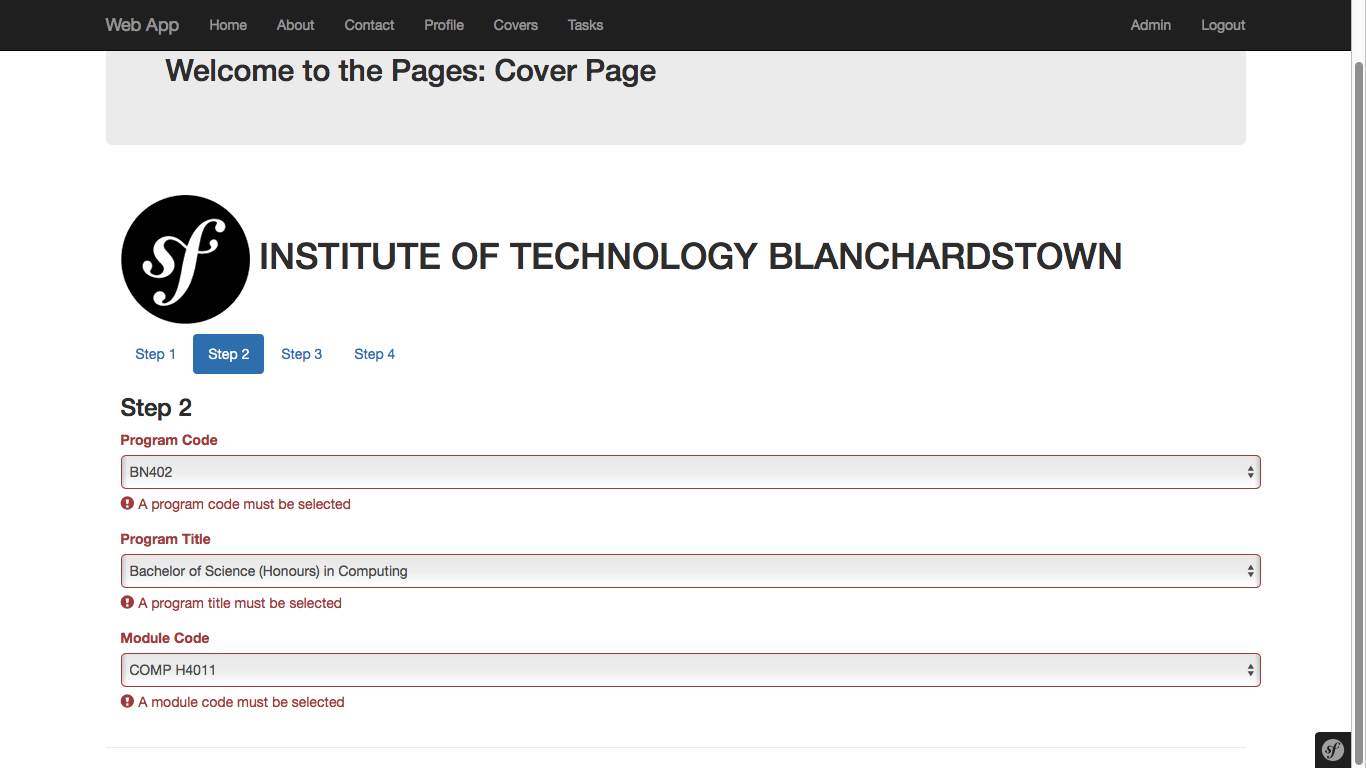
\includegraphics[width=400pt]{figures/step_2.png} % requires the graphicx package
   \caption{Cover Generation Step 2}
   \label{fig:Cover Generation Step 2}
\end{figure}

\begin{figure}[htbp]
   \centering
   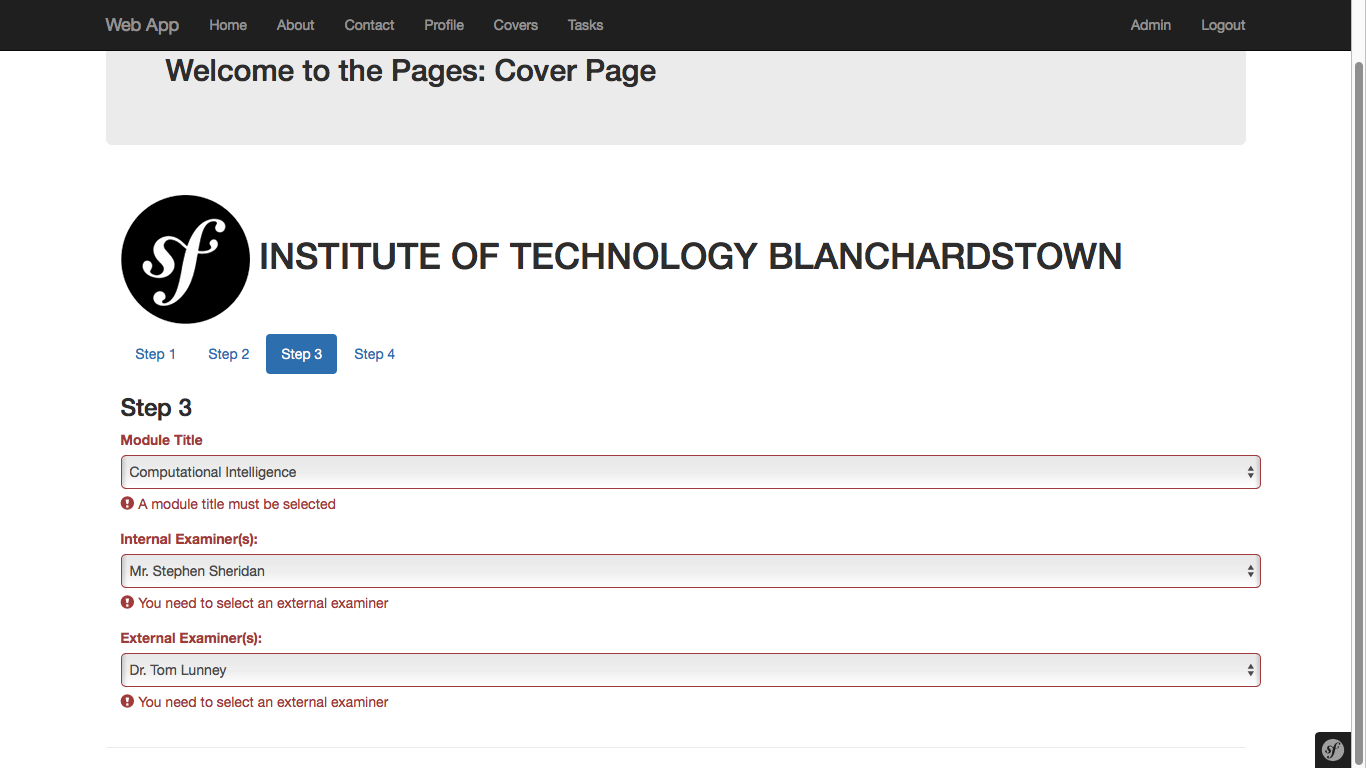
\includegraphics[width=400pt]{figures/step_3.png} % requires the graphicx package
   \caption{Cover Generation Step 3}
   \label{fig:Cover Generation Step 3}
\end{figure}

\begin{figure}[htbp]
   \centering
   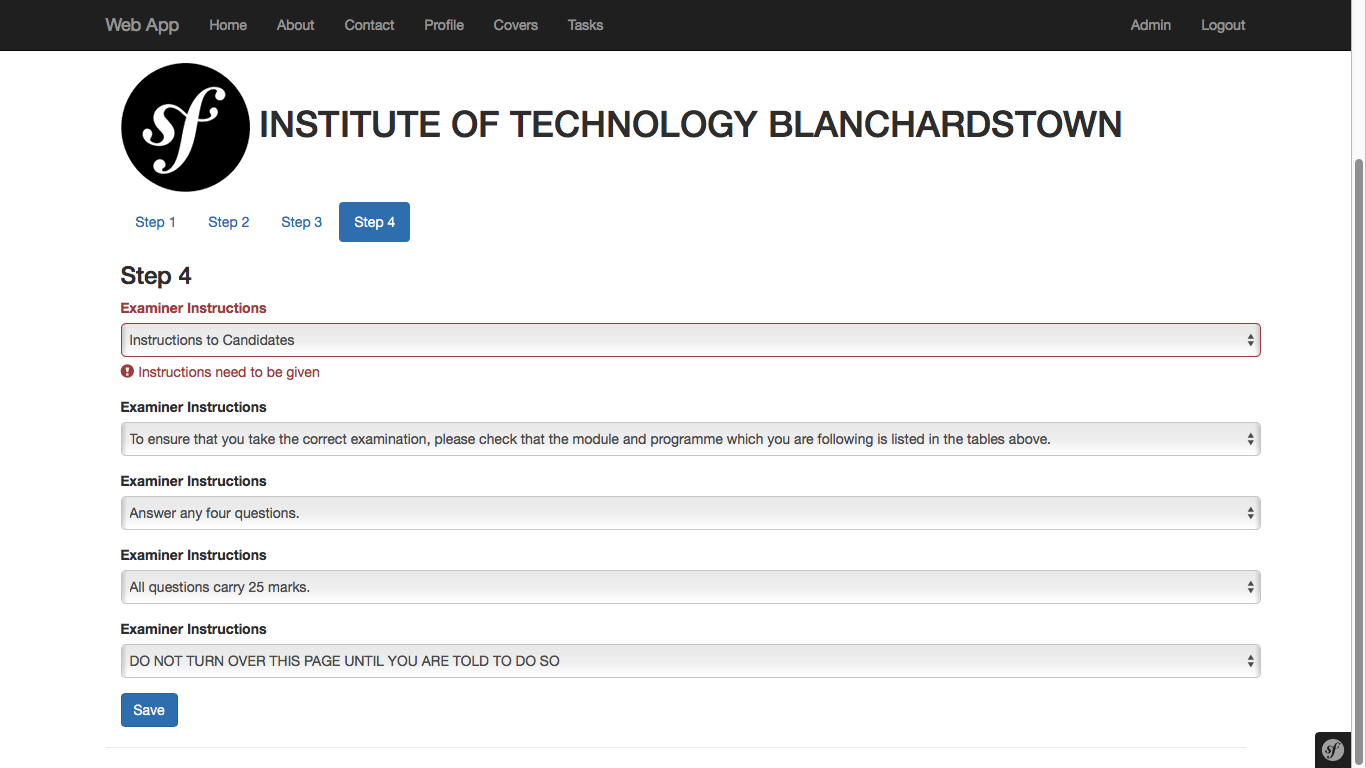
\includegraphics[width=400pt]{figures/step_4.png} % requires the graphicx package
   \caption{Cover Generation Step 4}
   \label{fig:Cover Generation Step 4}
\end{figure}

\begin{figure}[htbp]
   \centering
   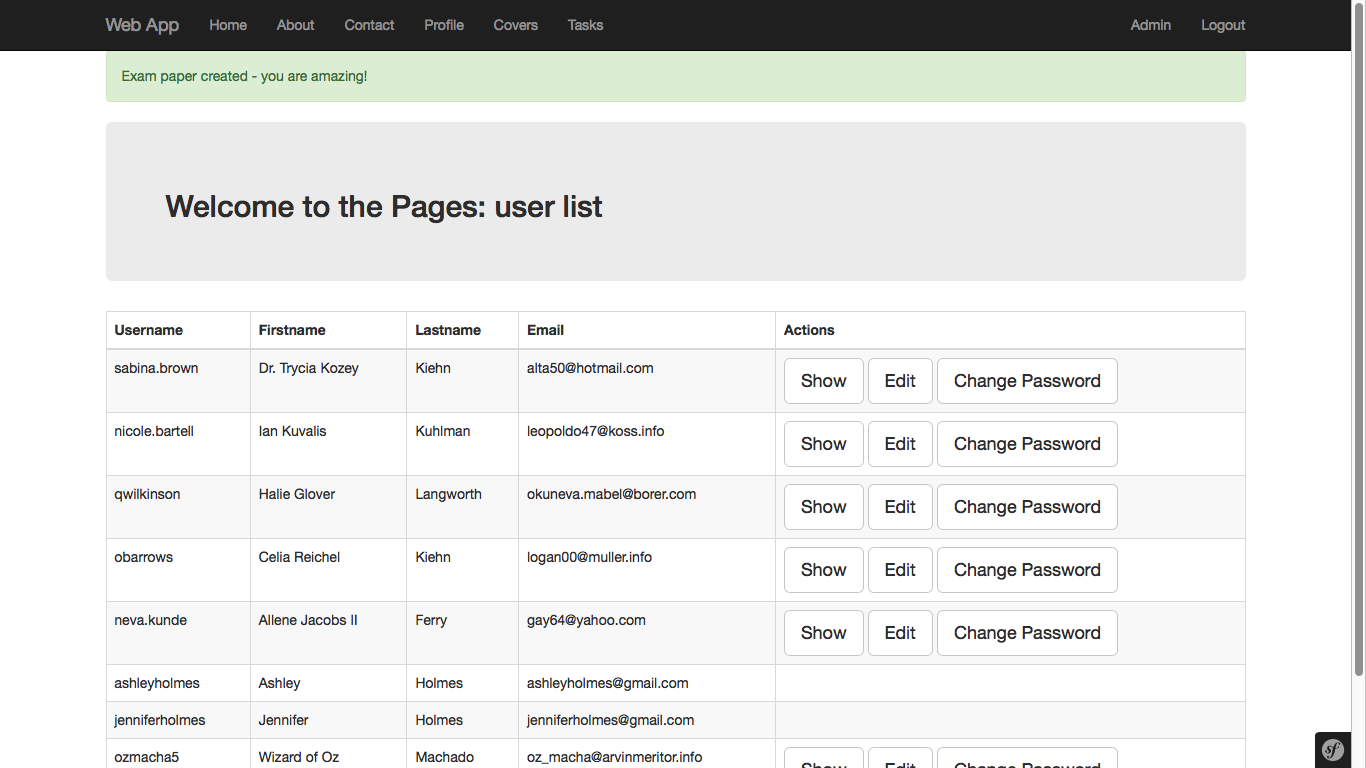
\includegraphics[width=400pt]{figures/exam_success.png} % requires the graphicx package
   \caption{Cover Page Successful}
   \label{fig:Cover Page Successful}
\end{figure}

\begin{figure}[htbp]
   \centering
   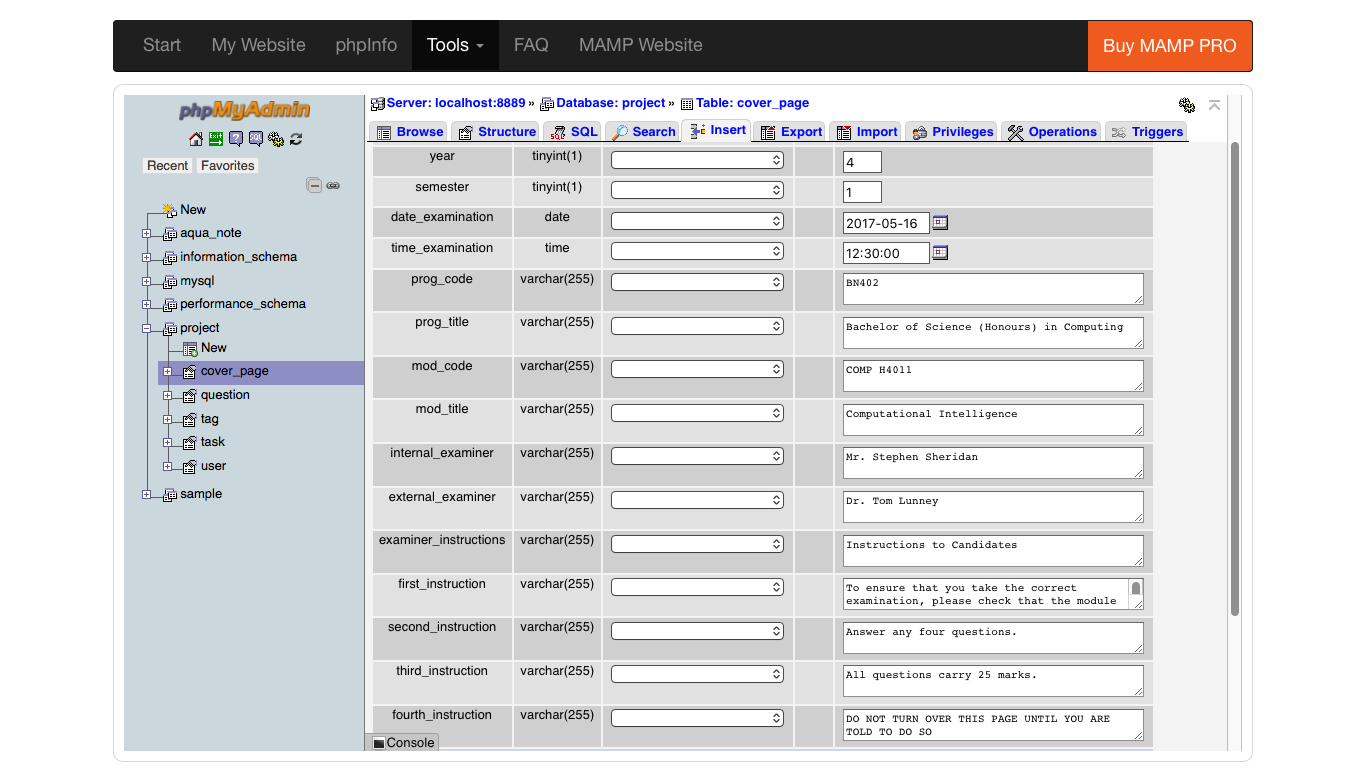
\includegraphics[width=400pt]{figures/exam_success_db.png} % requires the graphicx package
   \caption{Cover Page Successful DB}
   \label{fig:Cover Page Successful DB}
\end{figure}

\section{Testing Question Page}

\subsection{Successful Form Validation}

All the tests which were carried out on the previous form were also carried out on the question paper generation.

\begin{figure}[htbp]
   \centering
   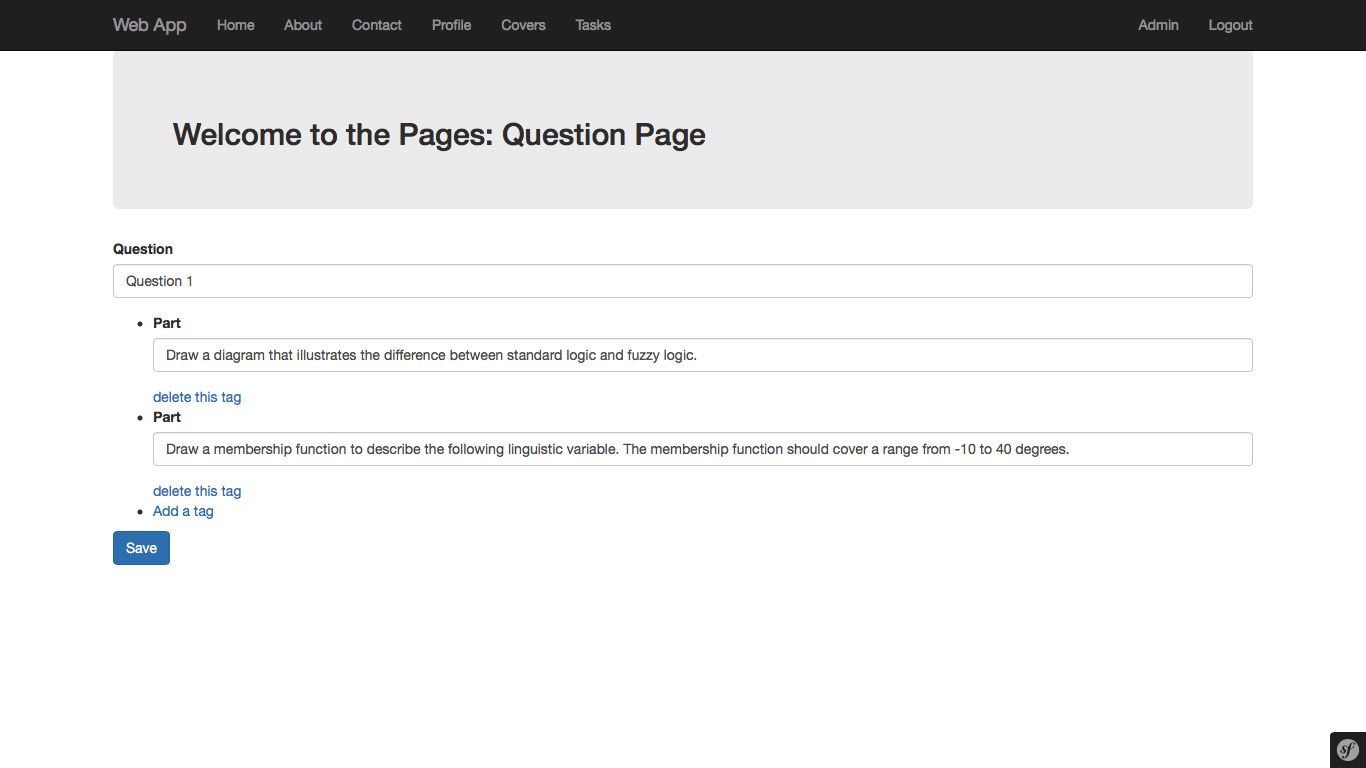
\includegraphics[width=400pt]{figures/tasks_test.png} % requires the graphicx package
   \caption{Question Page Successful}
   \label{fig:Question Page Successful}
\end{figure}

\begin{figure}[htbp]
   \centering
   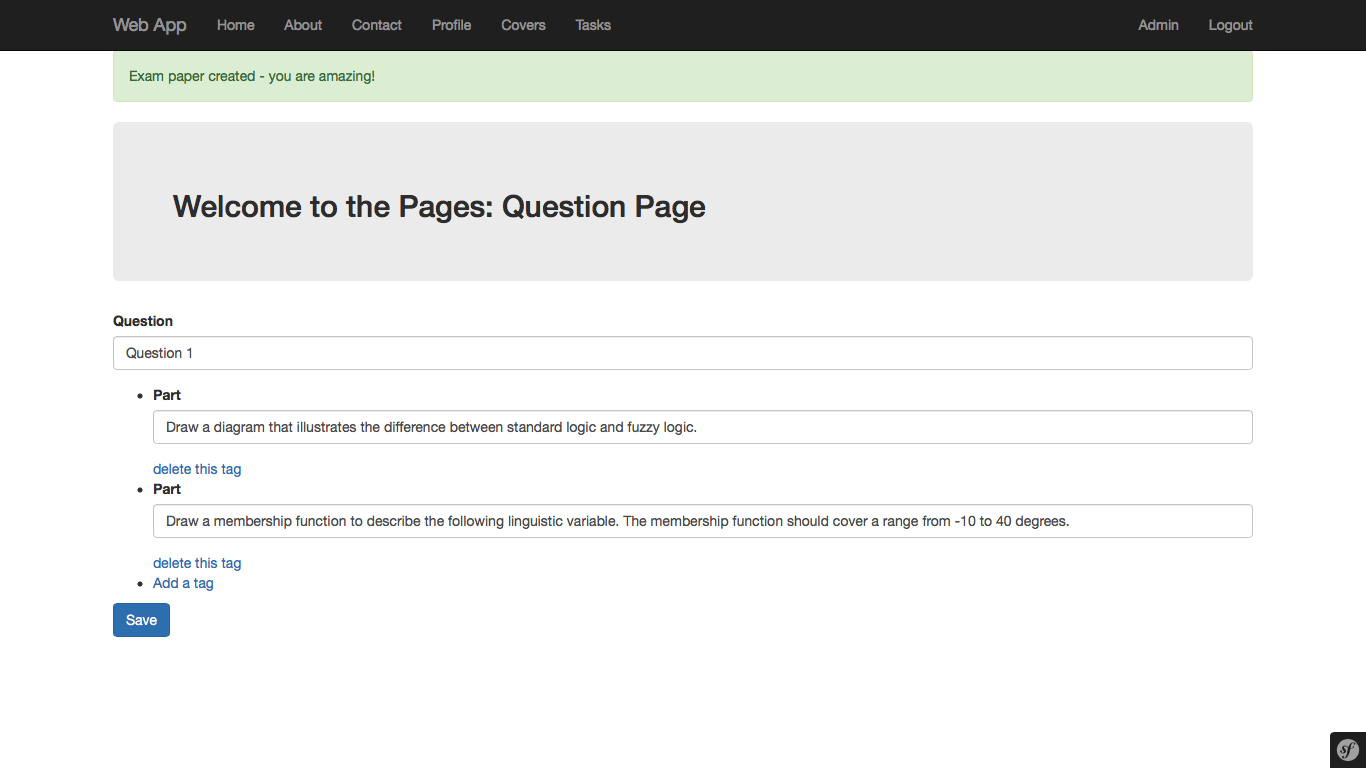
\includegraphics[width=400pt]{figures/tasks_success.png} % requires the graphicx package
   \caption{Question Page Successful DB}
   \label{fig:Question Page Successful DB}
\end{figure}

\begin{figure}[htbp]
   \centering
   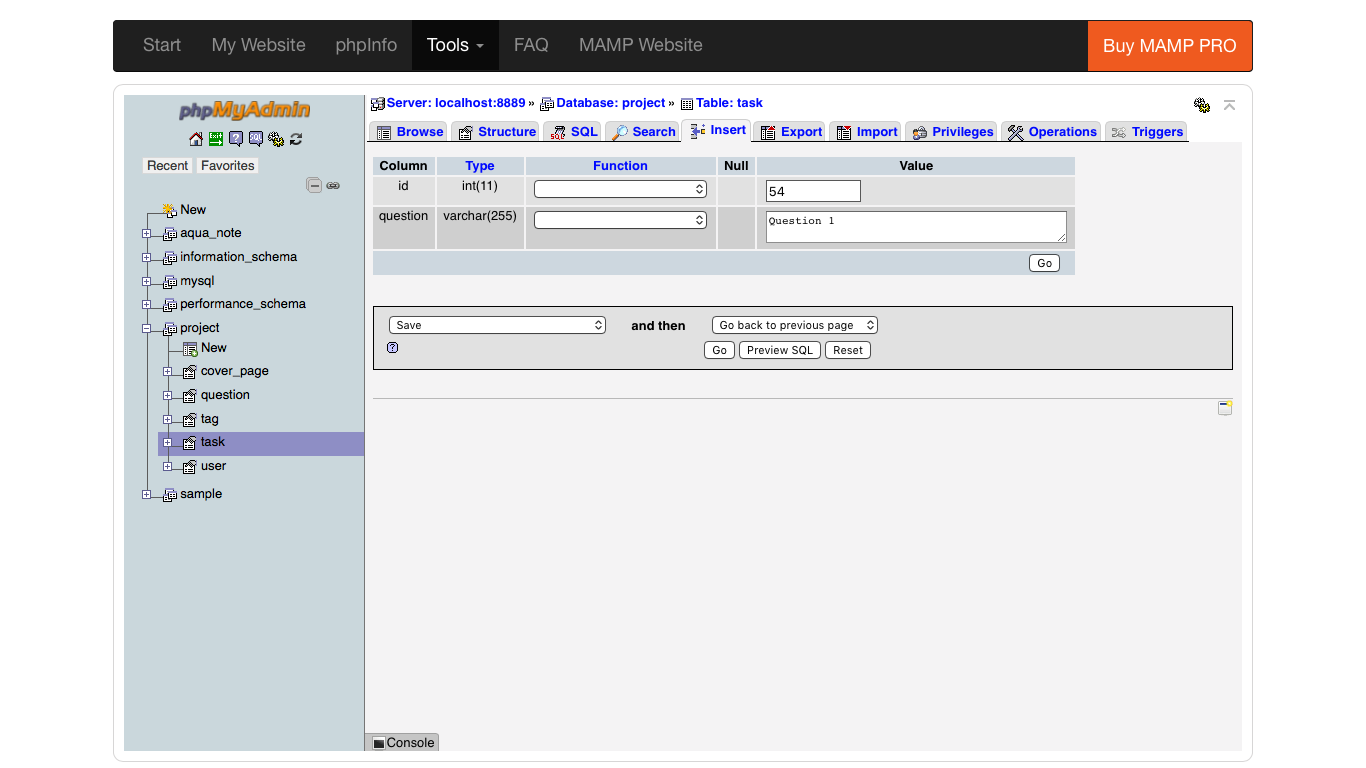
\includegraphics[width=400pt]{figures/tasks_question.png} % requires the graphicx package
   \caption{Question Page Metadata}
   \label{fig:Question Page Metadata}
\end{figure}

\begin{figure}[htbp]
   \centering
   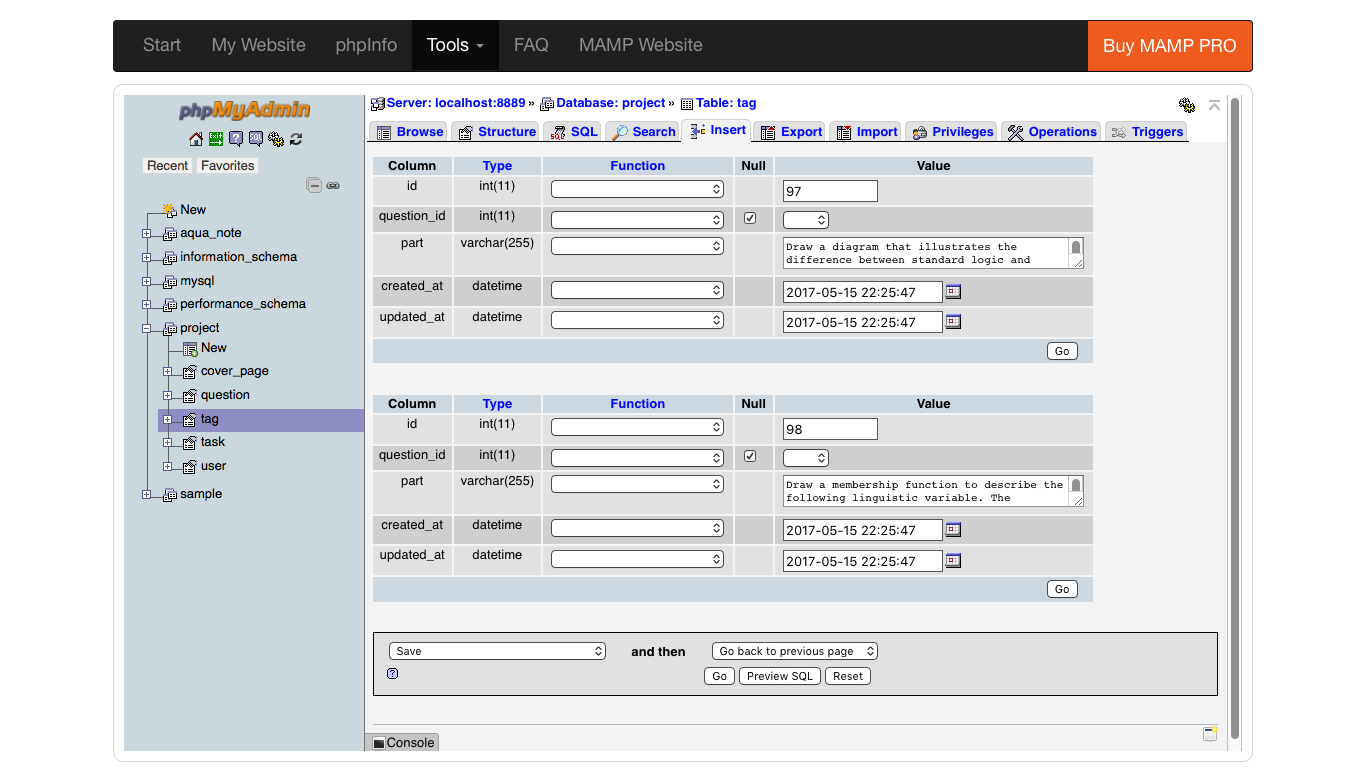
\includegraphics[width=400pt]{figures/tasks_question_db.png} % requires the graphicx package
   \caption{Cover Page Successful DB}
   \label{fig:Cover Page Successful DB}
\end{figure}

\begin{figure}[htbp]
   \centering
   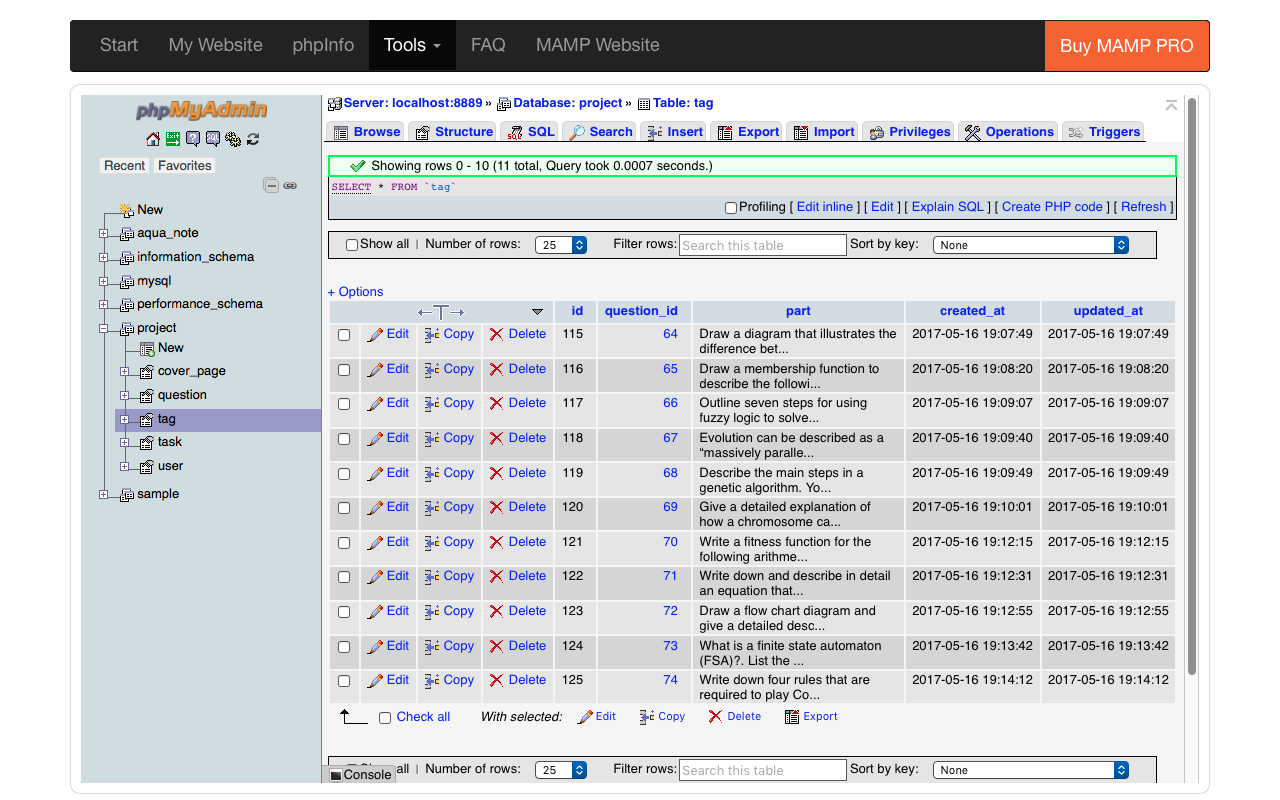
\includegraphics[width=400pt]{figures/historical_data.png} % requires the graphicx package
   \caption{Metadata from database}
   \label{fig:Metadata from database}
\end{figure}